\chapter{Foundations}

\section{Deep Learning}
\subsection{Neurons}

\subsection{Neural Networks}
\subsubsection{Activation Functions}
\subsubsection{Training Neural Networks}


\subsection{Convolutional Neural Networks}

A Convolutional Neural Network (CNN) is a deep neural network architecture designed to process grid-like data, especially images. CNNs are particularly effective for visual tasks because they exploit the spatial structure of an image and learn local patterns such as edges, corners, and textures. Unlike fully connected networks, CNNs do not treat every pixel independently. Instead, they use small learnable filters that are applied across the image to detect relevant structures at different positions.

\subsubsection{Convolution}

The main idea of a CNN is the convolution operation. In the case of a grayscale image, a small kernel is moved across the image and combined with the underlying pixel values. This produces a new image, called a feature map, which highlights the patterns detected by the kernel. Since the same kernel is reused at every spatial location, CNNs are able to detect the same feature independent of its position in the image.


\begin{figure}[h]
    \centering
    \subfigure[Original Image: No convolution is applied]{
        \parbox{4.6cm}{
            \centering
            {\small\textbf{Original}}\par
            \vspace{0.3em}
            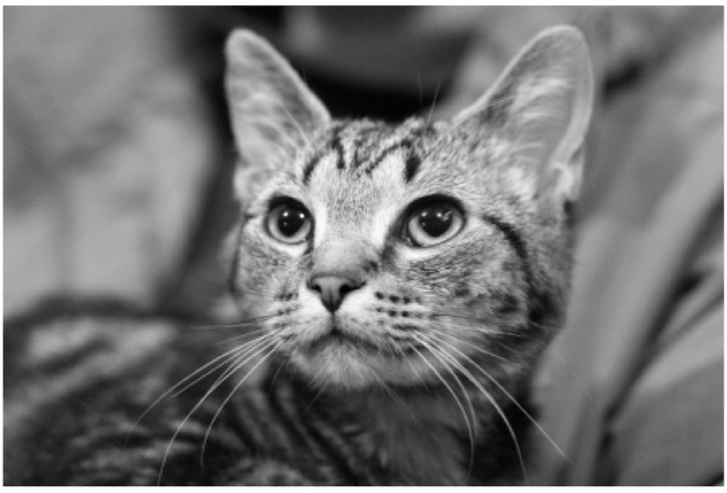
\includegraphics[width=4.5cm]{./chapter2/media/CNNCatPrewittOriginal_3}
        }
        \label{fig:CNNCatPrewittOriginal}
    }
    \hspace{0.3cm}
    \subfigure[Convolved Image, after the horizontal Prewitt kernel is applied to the original image]{
        \parbox{4.7cm}{
            \centering
            {\small\textbf{Horizontal Prewitt}}\par
            \vspace{0.3em}
            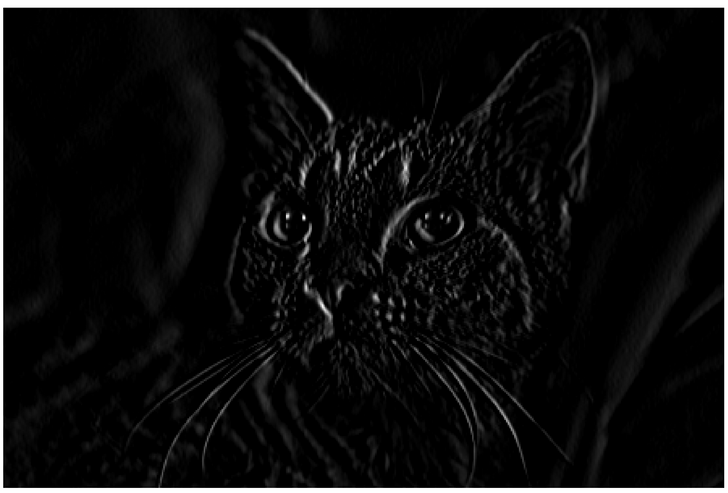
\includegraphics[width=4.5cm]{./chapter2/media/CNNCatPrewittHorizontal_3}
        }
        \label{fig:CNNCatPrewittHorizontal}
    }
    \hspace{0.3cm}
    \subfigure[Convolved Image, after the vertical Prewitt kernel is applied to the original image]{
        \parbox{4.6cm}{
            \centering
            {\small\textbf{Vertical Prewitt}}\par
            \vspace{0.3em}
            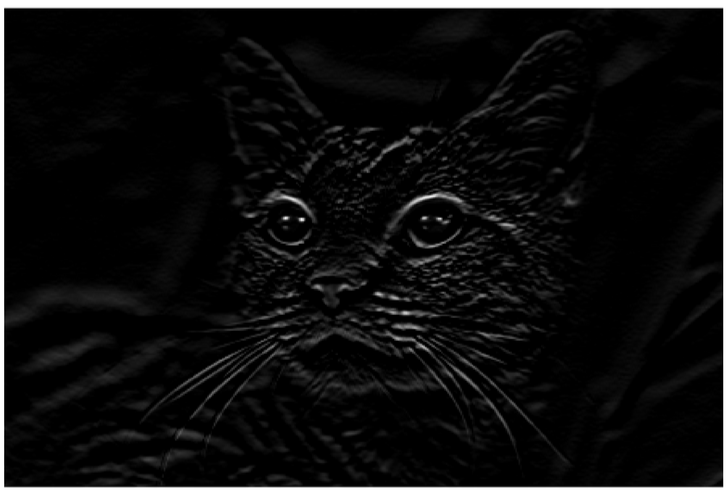
\includegraphics[width=4.5cm]{./chapter2/media/CNNCatPrewittVertical_3}
        }
        \label{fig:CNNCatPrewittVertical}
    }
    \caption[Image-based instructions for task execution.]{Image-based instructions for task execution. Image source: \cite{xxx}.}
    \label{fig:CNNCatPrewitt}
\end{figure}


For example, the Prewitt operator can be used to detect horizontal and vertical edges. The two $3 \times 3$ kernels are given by

\[
K_{\text{horizontal}} =
\begin{bmatrix}
-1 & 0 & 1\\
-1 & 0 & 1\\
-1 & 0 & 1
\end{bmatrix}
\qquad
K_{\text{vertical}} =
\begin{bmatrix}
-1 & -1 & -1\\
0 & 0 & 0\\
1 & 1 & 1
\end{bmatrix}
\]

By applying these kernels to the input image, two different feature maps are obtained: one emphasizing horizontal edges and one emphasizing vertical edges. More generally, different kernels extract different visual structures from the same image.

\begin{figure}
	\centering
	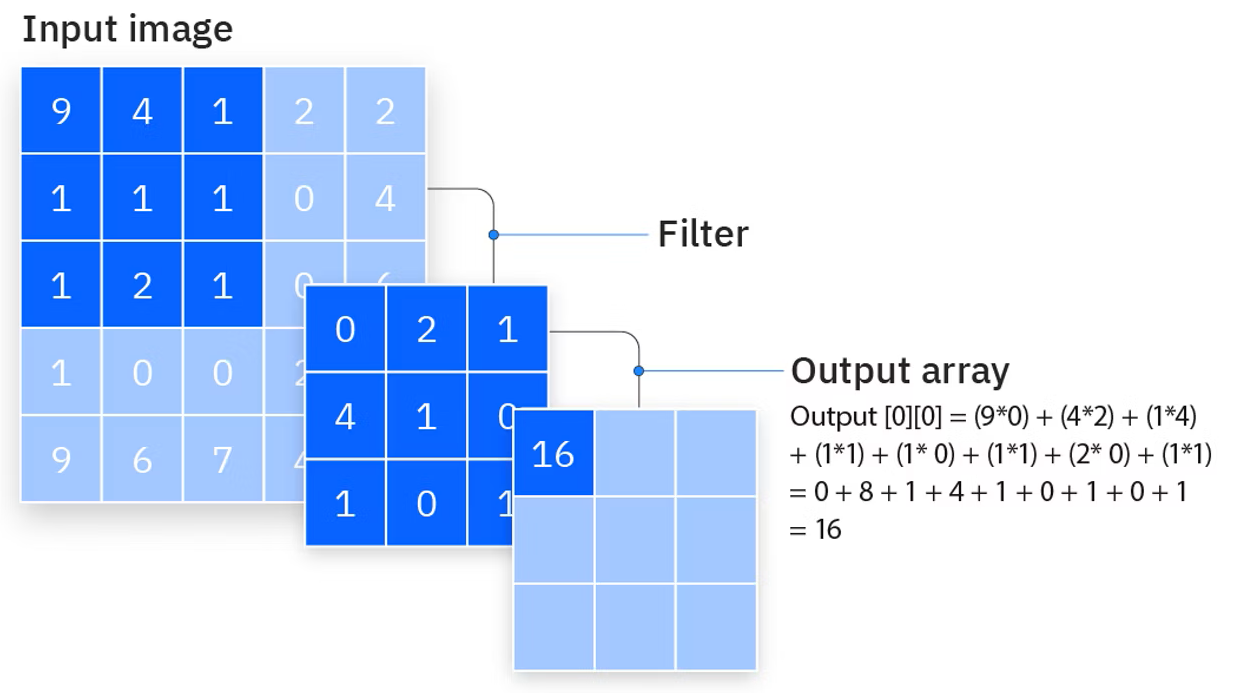
\includegraphics[width=0.65\linewidth]{./chapter2/media/CNNConvolutionIntro.png}
	\caption[CNN Convolution Introduction]{CNN Convolution Introduction. Image based on \cite{xxx}.}
	\label{fig:CNNConvolutionIntro}
\end{figure}

Mathematically, the convolution at position $(i,j)$ can be written as

\[
Y(i,j) = \sum_{u=-1}^{1}\sum_{v=-1}^{1} X(i+u,j+v)\cdot K(u+1,v+1),
\]

where $X$ is the input image, $K$ is the kernel, and $Y$ is the resulting feature map. In practice, the kernel is slid across the image step by step, and at each location the element-wise products are summed to obtain one output value.

To preserve the spatial resolution of the input image, padding is often added around the border before applying the convolution. With zero-padding, the image size can remain unchanged after the convolution, which is useful when multiple convolution layers are stacked. Importantly, the kernels are not fixed manually in a CNN. Instead, they are learned during training, allowing the network to adapt its filters to the task at hand.

\begin{figure}
	\centering
	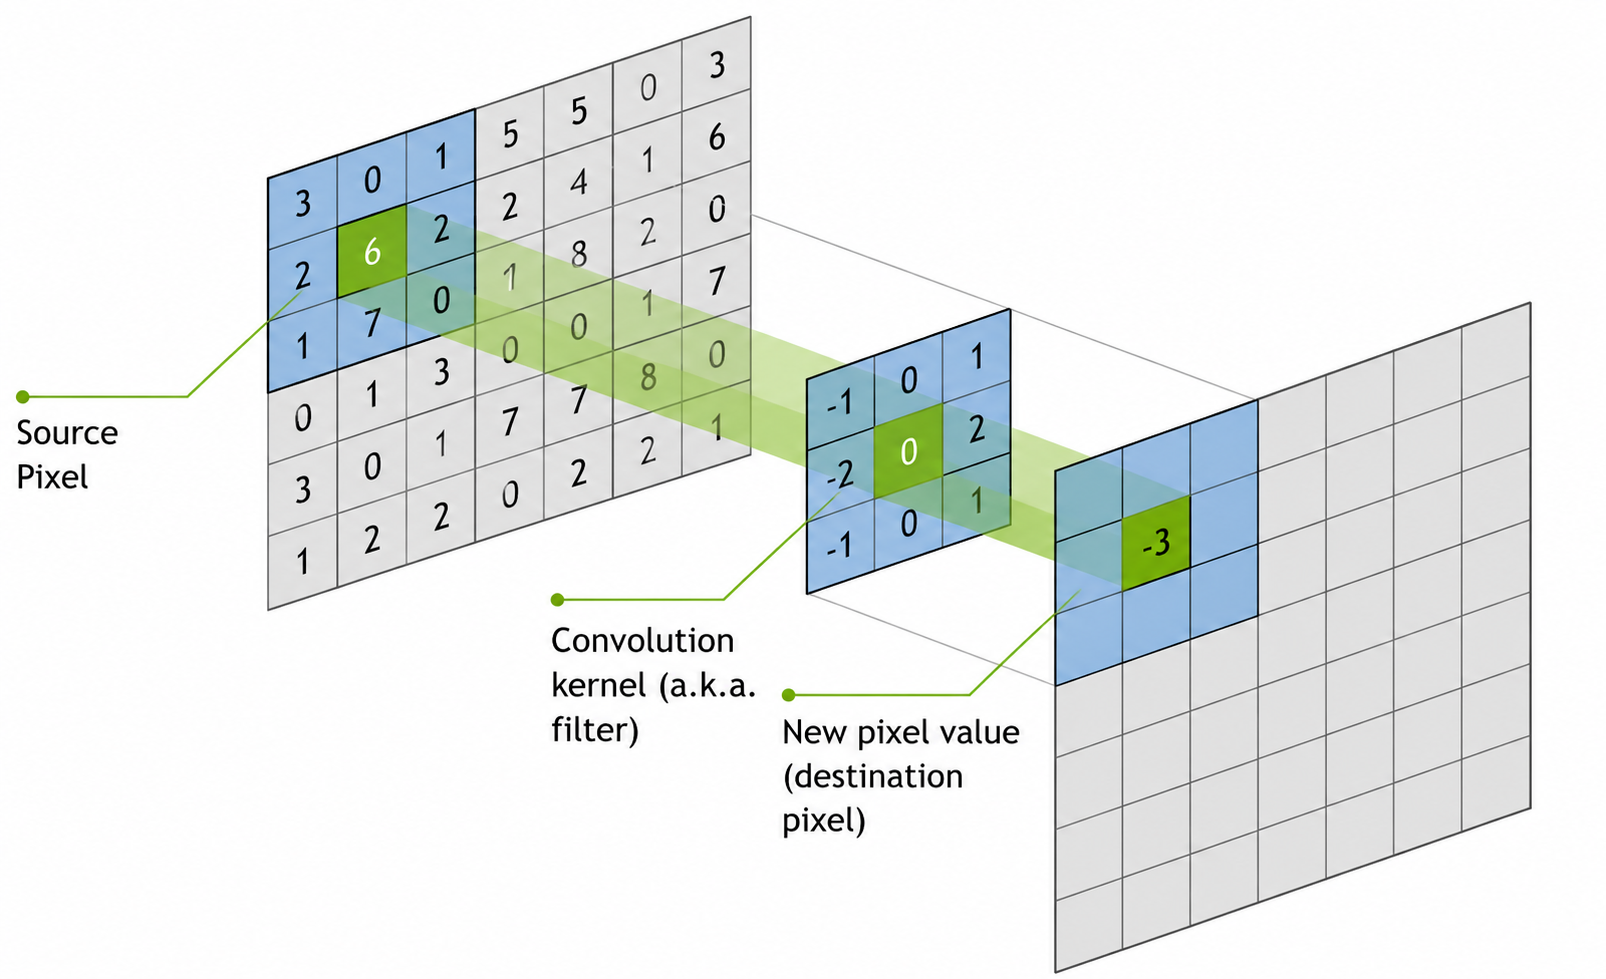
\includegraphics[width=0.65\linewidth]{./chapter2/media/CNNConvolutionIntro_View2}
	\caption[CNN Convolution Introduction]{CNN Convolution Introduction. Image based on \cite{xxx}.}
	\label{fig:CNNConvolutionIntro_View2}
\end{figure}


\begin{figure}
	\centering
	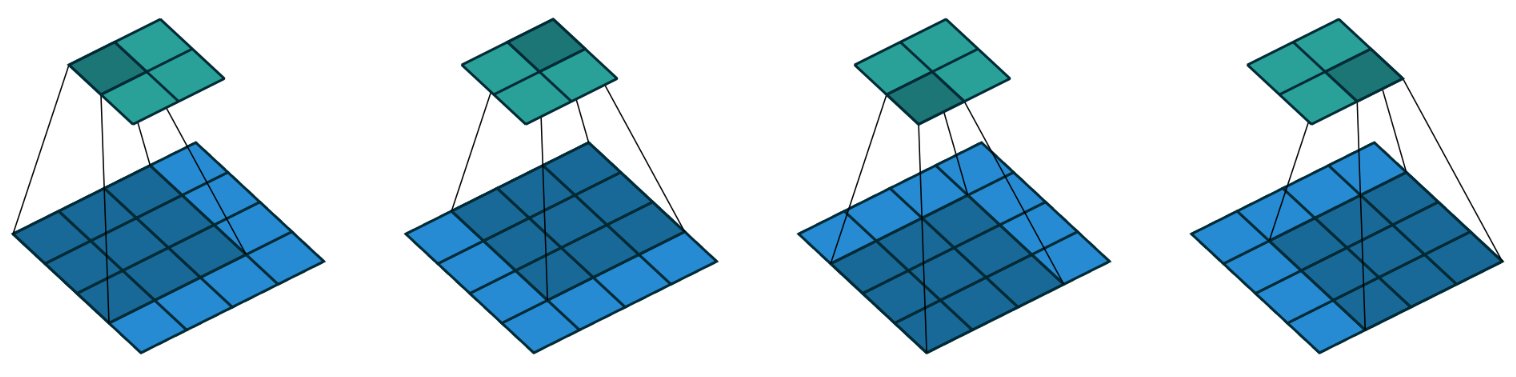
\includegraphics[width=0.9\linewidth]{./chapter2/media/CNNConvolution_1}
	\caption[CNN Convolution Introduction]{CNN Convolution Introduction. Image based on \cite{xxx}.}
	\label{fig:CNNConvolutionIntro_View2}
\end{figure}

\begin{figure}
	\centering
	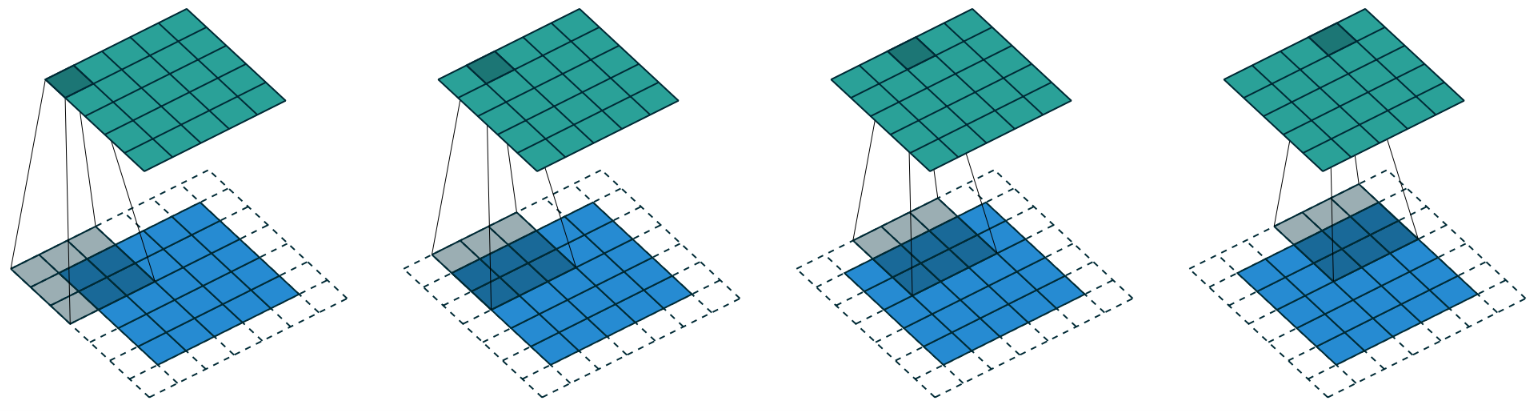
\includegraphics[width=0.9\linewidth]{./chapter2/media/CNNConvolution_1_withPadding}
	\caption[CNN Convolution Introduction]{CNN Convolution Introduction. Image based on \cite{xxx}.}
	\label{fig:CNNConvolutionIntro_View2}
\end{figure}




% \begin{figure}
% 	\centering
% 	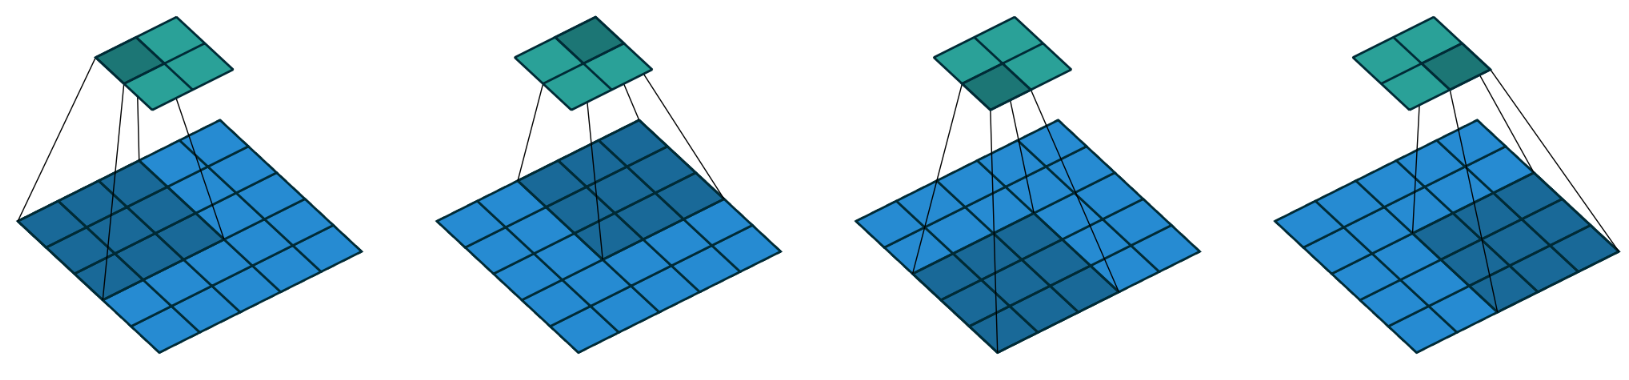
\includegraphics[width=0.65\linewidth]{./chapter2/media/CNNConvolution_1_withStride2}
% 	\caption[CNN Convolution Introduction]{CNN Convolution Introduction. Image based on \cite{Vaswani2017AttentionIA}.}
% 	\label{fig:CNNConvolutionIntro_View2}
% \end{figure}


% \begin{figure}
% 	\centering
% 	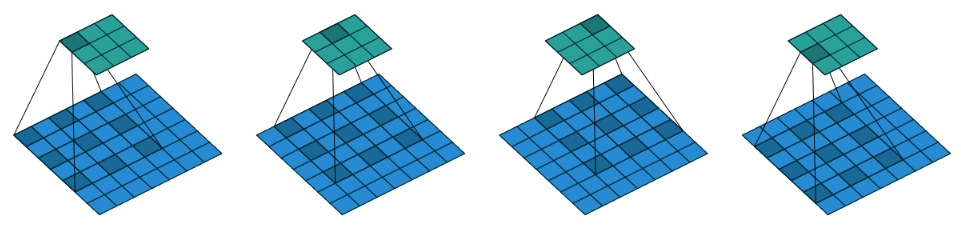
\includegraphics[width=0.65\linewidth]{./chapter2/media/CNNConvolution_1_withDilation}
% 	\caption[CNN Convolution Introduction]{CNN Convolution Introduction. Image based on \cite{Vaswani2017AttentionIA}.}
% 	\label{fig:CNNConvolutionIntro_View2}
% \end{figure}


\subsubsection{Pooling}

\begin{figure}
	\centering
	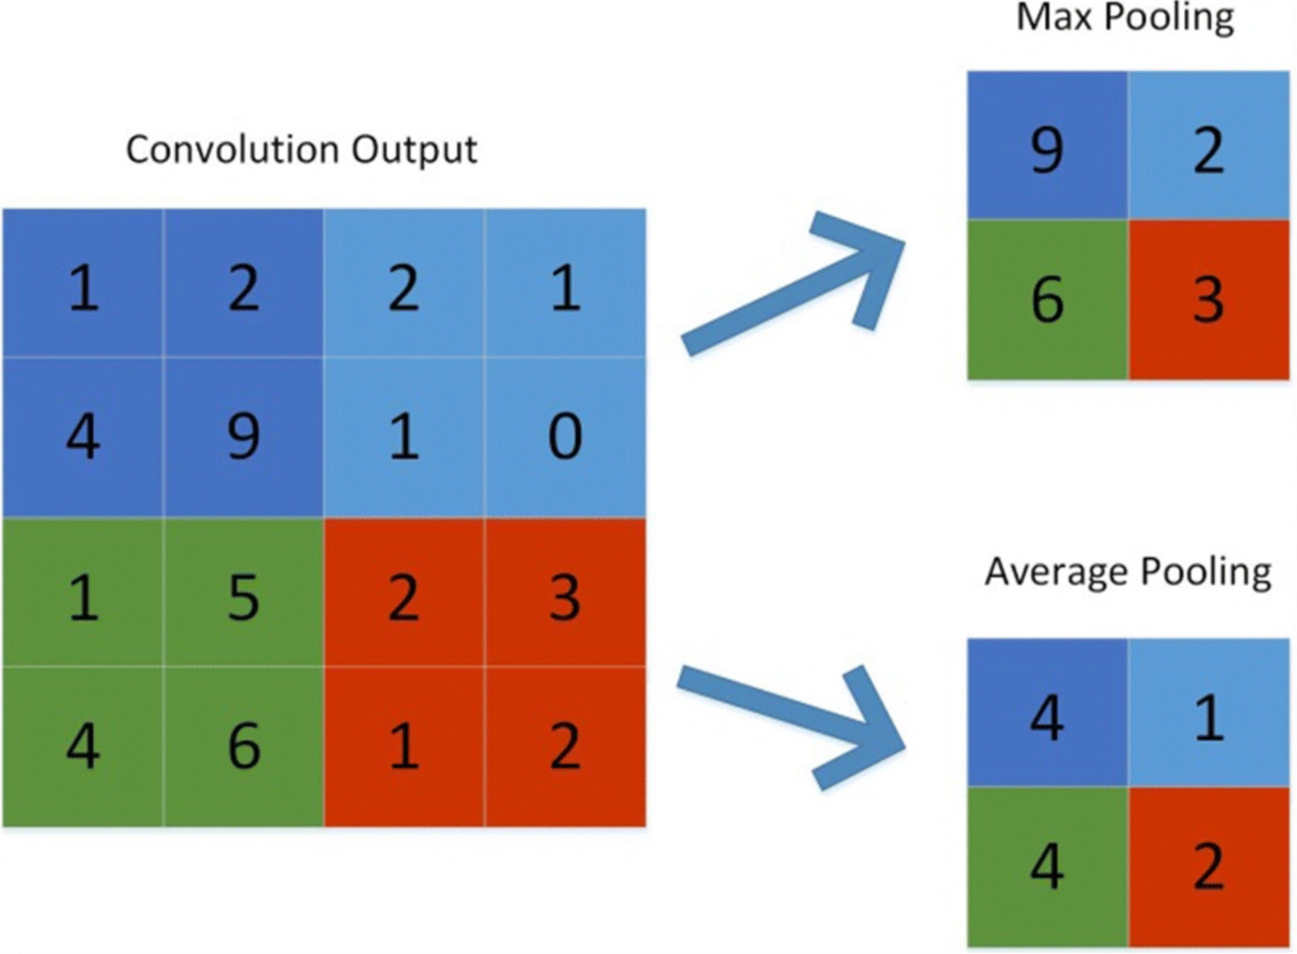
\includegraphics[width=0.45\linewidth]{./chapter2/media/CNNPooling}
	\caption[CNN Pooling]{CNN Pooling. Image based on \cite{xxx}.}
	\label{fig:CNNPooling}
\end{figure}


Another central component of CNNs is the pooling layer. Pooling reduces the spatial size of the feature maps while retaining the most important information. This lowers the computational cost and increases robustness to small shifts in the input image.

In max pooling, the maximum value within a local region is selected. In average pooling, the mean value of the region is computed. Both methods summarize local neighborhoods, but max pooling is more commonly used in practice because it preserves the strongest activation. Pooling is typically applied after convolution layers and helps the network build increasingly compact and informative representations.

\subsubsection{CNN Pipeline}

A CNN usually consists of several repeated blocks of convolution and pooling layers. Early layers detect simple features such as edges and corners, while deeper layers combine these basic features into more complex structures. After several convolution and pooling stages, the feature maps are flattened and passed through fully connected layers or a classification head to produce the final output.

In this thesis, the convolution operation is first explained for a grayscale image to illustrate the basic principle. The same idea can then be extended to RGB images, where the kernels operate across all color channels.

\begin{figure}
	\centering
	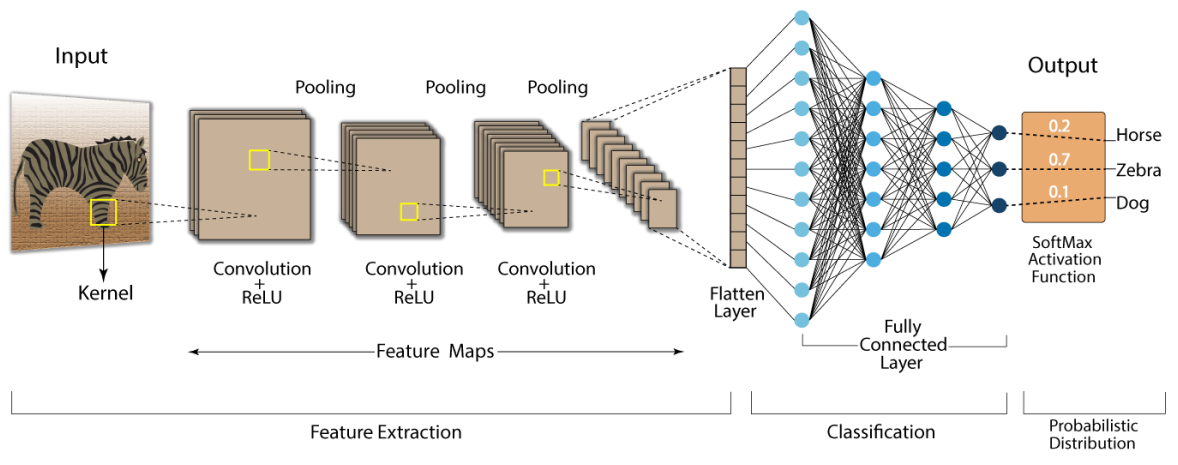
\includegraphics[width=1.0\linewidth]{./chapter2/media/CNNPipeline}
	\caption[CNN Pipeline]{CNN Pipeline. Image based on \cite{xxx}.}
	\label{fig:CNNPipeline}
\end{figure}



